\section{S3 -- Asynchroniczna komunikacja serwerem HTTP w technologii AJAX}

Nazwa AJAX (Asynchronous JavaScript and XML) została wymyślona w 2005 roku. Miała ona opisywać istotę nowych narzędzi udostępnionych przez firmę Google (Google Suggest i Google Maps). Nie jest to oficjalna technologia tzn. nie ma na to standardu opisanego w RFC lub innym tego typu dokumencie. Określenie AJAX opisuje współdziałanie kilku technologii – języka JavaScript, protokołu http, mechanizmów przeglądarek internetowych i serwerów sieciowych. Generalnie AJAX mówi o asynchronicznej komunikacji z serwerem http, zapewniając pobieranie i wyświetlanie materiałów bez konieczności przeładowywania całej strony. Sama nazwa może być myląca, nie trzeba rozumieć XML, aby zrozumieć AJAX.

\textbf{Czym różni się komunikacja asynchroniczna od komunikacji synchronicznej?}

Komunikacja synchroniczna, to standardowy sposób komunikacji, kiedy to wysyłając zadanie blokując czekamy ze zwróceniem interfejsu do klienta, aż zadanie zostanie przetworzone. W przypadku krótkich transakcji taka sytuacja jest do przyjęcia, jednak w przypadku bardzo długich transakcji nie ma ona racji bytu. 
\begin{figure}[H]
\centering
\caption{Komunikacja synchroniczna}
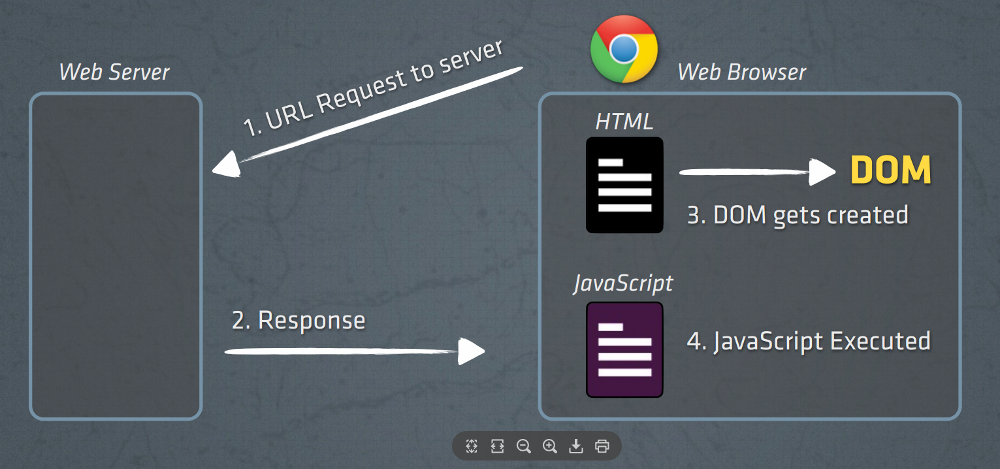
\includegraphics[width=\linewidth]{s3_int_kom_synchr.png}
\end{figure}

Komunikacja asynchroniczna pozwala nam wysyłać zapytanie w tle bez konieczność czekania ze zwróceniem interfejsu klienta. Kiedy zapytanie się skończy zostanie wywołana wcześniej zdefiniowana funkcja. Dzięki temu możemy:
\begin{itemize}
\item aktualizować zawartość strony przez konieczności przeładowywania całego drzewa DOM. 
\item wysyłać dane do serwera po załadowaniu się całej strony;
\item otrzymywać odpowiedź od serwera po załadowaniu się całej strony;
\item wysyłać dane do serwera w tle
\end{itemize}

\begin{figure}[H]
\centering
\caption{Komunikacja asynchroniczna}
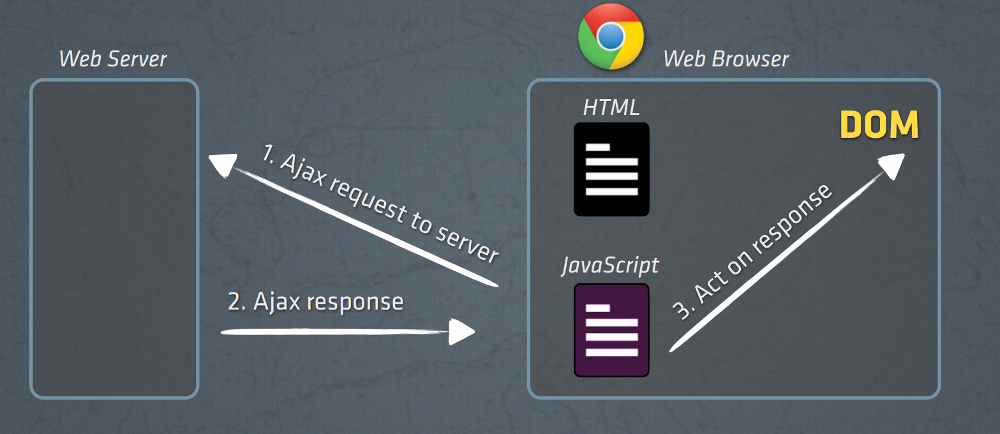
\includegraphics[width=\linewidth]{s3_int_kom_asynchr.png}
\end{figure}

Przykłady zastosowań AJAX:
\begin{itemize}
\item Wyświetlanie nowych danych HTML bez konieczności odświeżania strony;
\item Przesyłanie formularzy i natychmiastowe wyświetlanie wyników;
\item Logowanie bez opuszczania strony;
\item Kontrolka do oceny materiałów za pomocą liczby gwiazdek;
\item Przeglądanie informacji z bazy danych.  
\end{itemize}

Co jest nam potrzebne do rozpoczęcia działania? 
\begin{itemize}
\item \textbf{Przeglądarka internetowa} -- wbudowany obiekt XMLHttpRequest -- wprowadzony w przeglądarce Internet Explorer 5;
\item \textbf{Język JavaScript} -- wykonywanie zadań w AJAX-ie np. wysyła żądania na serwer, oczekuje i przetwarza odpowiedź, aktualizuje stronę przez dodanie nowych materiałów lub zmianę jej wyglądu
\item \textbf{Serwer Sieciowy} -- odbiera zadanie od przeglądarki i przesyła odpowiedź z danymi.
\end{itemize}
\begin{figure}[H]
\centering
\caption{Klasyczne AJAX-owe przetwarzanie}
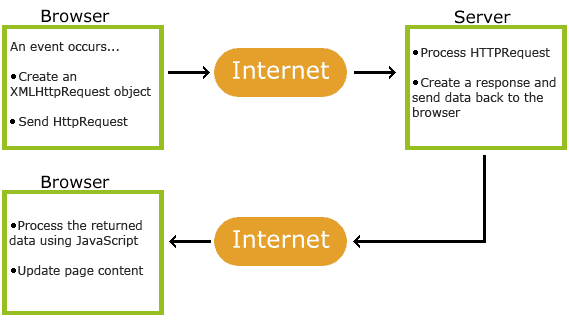
\includegraphics[width=0.8\linewidth]{s3_int_ajax_przetwarzanie.png}
\end{figure}

Implementacja zapytań ASYNCHRONICZNYCH w czystym JavaScripcie:
\begin{enumerate}
\item Utworzenie obiektu XMLHttpRequest (dostępny natywnie w przeglądarkach) -- więcej informacji \url{https://developer.mozilla.org/pl/docs/XMLHttpRequest}
\item Specyfikacja typu zapytania -- funkcja \texttt{open(method, url, async)};
\item Specyfikacja zdarzenia \texttt{onreadystatechange}:
\begin{enumerate}
\item pole obiektu XMLHttpRequest przechowuje funkcję, która jest automatycznie wywoływana kiedy \texttt{readyState} zmienia się;
\item pole \texttt{readyState} przechowuje status żądania HTTP zmieniającego się od 0 --- 4
\begin{enumerate}
\item 0 -- zapytanie niezainicjalizowane;
\item 1 -- nawiązanie połączenia z serwerem;
\item 2 -- zapytanie zostało otrzymane;
\item 3 -- przetwarzanie zapytania;
\item 4 -- zapytanie przetworzone, odpowiedź otrzymana;
\end{enumerate}
\end{enumerate}
\item Wysłanie zapytania funkcja send:
\begin{enumerate}
\item \texttt{send()} -- wysyła zapytanie wykorzystując GET;
\item \texttt{send(string)} -- wysyła dane na serwer;
\end{enumerate}
\end{enumerate}

\textbf{Obiekty promise -- JavaScript}
Obiekt promise jest używany do zadań asynchronicznych i odroczonych w czasie. Reprezentuje operację, która nie została jeszcze zakończona, ale oczekuje na zakończenie w przyszłości. Obiekt może znajdować się w 3 stanach:
\begin{itemize}
\item \texttt{pending} -- początkowy stan obiektu promise;
\item \texttt{fulfilled} -- stan reprezentujący operację zakończoną powodzeniem;
\item \texttt{rejected} -- stan reprezentujący operację zakończoną niepowodzeniem;
\end{itemize}
Obiekty promise wykorzystują do zapytań asnychronicznch biblioteki i frameworki webowe np. jQuery oraz AngularJS.


